%%=============================================================================
%% Methodologie
%%=============================================================================

\chapter{\IfLanguageName{dutch}{Proof of concept}{Proefafdruk}}
\label{ch:Proof of concept}

Het doel van dit hoofdstuk is om een idee te creëren van de omgeving waarin Cisco Identity Services Engine is geïmplementeerd. Een uitgebreide uitleg over de elementen die aanwezig zijn binnen de omgeving van Cisco is in dit hoofdstuk terug te vinden. Ieder hardwareapparaat is zorgvuldig beschreven waarbij informatie is te vinden over de specificatie, de configuraties en de instellingen van de hardware componenten. Daarnaast zijn ook de implementaties van de virtuele machines verder toegelicht.
\newline
\newline
Samen met deze informatie zijn belangrijke schema’s verwerkt in dit hoofdstuk die een visueel beeld geven over dit afgezonderd netwerk. 
Vervolgens is er de sectie die de enquête bespreekt. De bespreking van de enquête bevat voornamelijk informatie die in sectie \ref{sec:enquête} terug te vinden is. 

\section{Cisco Identity Services Engine omgeving}

Voor de implementaties en proeven van Cisco Identity Services Engine en zijn benodigde use cases is er een omgeving vereist. Deze omgeving is voorzien door een Belgische aanbieder van digitale televisie, internet, mobiele telefonie, die gekend is als Telenet Group N.V. Implementaties en de proeven van Cisco Identity Services Engine en met zijn benodigde use cases is uitgewerkt in een Telenet thuisnetwerk.
\newline
Om de essentiële componenten van dit thuisnetwerk te beschermen tegen breuk, is de implementatie verder uitgewerkt in een afgezonderd netwerk. Dit wordt mogelijk gemaakt met behulp van een virtuele opensource router/firewall zoals Pfsense. Dit virtuele routertje dient als gateway voor de verschillende vlan’s waarbij het thuisnetwerk gebruikt zal worden als ‘uplink’ naar het internet. 



\subsection{Server VMware ESXi}
Het afgezonderd netwerkje bestaat uit een rack server waarop een vijftal virtuele machines draaien. Deze virtuele machines zijn: Cisco Identity Services Engine, het virtuele Pfsense routerje, en drie Windows Server 2019 datacenters machines. Dit wordt eenvoudig weergegeven in figuur \ref{fig:vms} die de virutele machines weergeeft. De creatie van deze virtuele machines is mogelijk gemaakt door VMware ESXi.  VWware ESXi is een type-1 hypervisor van enterprise-klasse, ontwikkeld door VMware voor het inzetten en bedienen van virtuele machines(\cite{VMwareESXI}). 
\newline
\newline
De ESXi server is geconfigureerd door het gebruik van een ‘bootable usb’. Deze bootable usb bevatte al nodige software om de server te voorzien met VMware ESXi. Vervolgens werd de server geconfigureerd met een aantal belangrijke settings, zoals het instellen van een ip adres, subnet mask, raid controller, enz. Hierbij zijn volgende settings op deze ESXi server voorzien: 

\begin{itemize}
	\item IP adres: 192.168.0.183
	\item Subnet: 255.255.255.0
	\item Default gateway: 192.168.0.1
	\item raid controller: RAID 10
\end{itemize}

\begin{figure}[H]
	\centering
	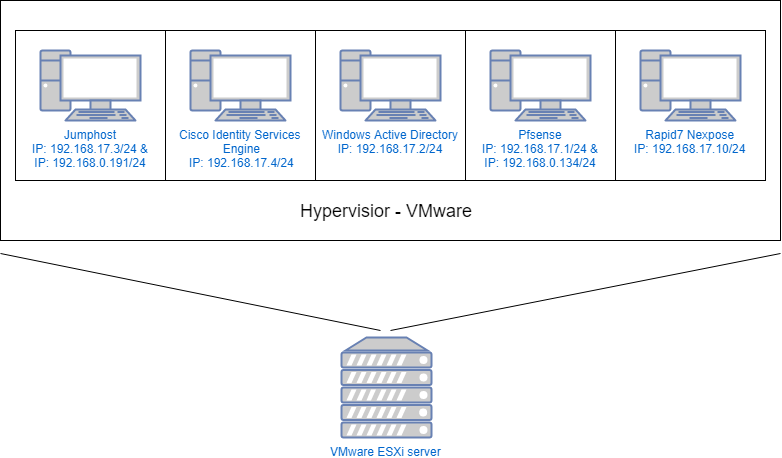
\includegraphics[width=0.9\textwidth]{servervm.png}
	\caption{Virtuele machines in VMware ESXi server}
	\label{fig:vms}
\end{figure}

\newpage
Door de configuratie van deze IP instellingen, is de VMware ESXi server toeganglijk via de webbrowser. Virtuele machines kunnen via de webbrowser beheerd, verwijderd en gecreëerd worden. Daarnaast werd de hard disk drive ingesteld met een RAID controller. RAID, een afkoring voor Redundant array of independent disks is een dataopslagtechnologie waarbij meerdere harde schijven gecombineerd worden tot één of meer logische virtuele opslageenheden. Dit heeft als doel om de veiligheid, snelheid en de capaciteit te kunnen vergroten. Hierbij is op de VMware ESXi RAID 10 geconfigueerd. RAID 10 is een hybride combinatie tussen RAID 1 en RAID 0. Waarbij men de snelheid van striping met de veiligheid van mirroring combineert(\cite{RAIDLi}). 
\newline
\newline
Dit is de veiligste en snelste methode maar ook het duurste. Het is een dure methode omdat er gebruik wordt gemaakt van RAID 1. Er is dus voor iedere 1TB aan opslagruimte ook 1TB aan mirror ruimte nodig, in combinatie met RAID 0 waardoor er veel fysieke harde schijven nodig zijn. In figuur \ref{fig:Raid10} wordt een voorbeeld van een RAID 10 schema weergegeven.

\begin{figure}[H]
	\centering
	\includegraphics[width=0.75\textwidth]{Raid10.png}
	\caption{Voorbeeld configuratieschema RAID 10 (\cite{Raid10}).}
	\label{fig:Raid10}
\end{figure}
\newpage
Vervolgens zijn er in de VMware ESXi server opstelling drie van de vier fysieke Ethernet adapters gebruikt. De adapters zijn op hun beurt verbonden met een virtuele switch. Elke fysieke adapter heeft een andere functie die in de onderstaande lijst zijn weergegeven. 

\begin{itemize}
	\item vmnic0, is de fysieke adapter die verbonden is met de virtuele switch, genaamd 'VSwitch0'.
	\item vmnic2, is de fysieke adapter die verbonden is met de virtuele switch, genaamd 'Sub\textunderscore switch'.
	\item vmnic3, is de fysieke adapter die verbonden is met de virtuele switch, genaamd 'Cisco \textunderscore switch'.
\end{itemize}

\subsubsection{Virtuele switches}
\subsubitem{\bf VSwitch0}
\newline
De 'VSwitch0' is een virtuele switch die voorzien is om de VMware ESXi server te contacteren via de webbrowser. Op figuur \ref{fig:Vswitch0} ziet men dat de 'VSwitch0' is ingesteld met vlan id 0, dat geen vlan identificatie voorziet. 
\newline
\newline
TCP/IP pakketen passeren deze interface wanneer gebruikers surfen naar "https://192.168.0.183". Vervolgens passeert de TCP/IP pakketen langs vmnic0 die de informatie doorgeeft aan de VSwitch0. Wanneer de informatie terecht komt op de VSwitch0, stuurt hij dit op zijn beurt door naar de VMKernel poort.


\begin{figure}[H]
	\centering
	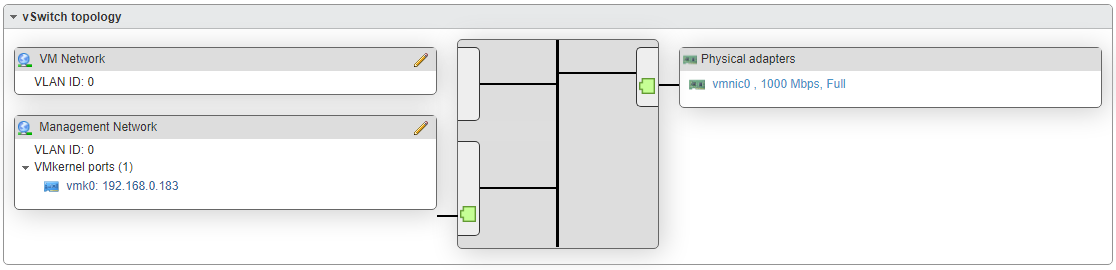
\includegraphics[width=0.9\textwidth]{VSwitch0.png}
	\caption{Topologie van de 'VSwitch0'}
	\label{fig:Vswitch0}
\end{figure}
\newpage
\subsubitem{\bf Sub\textunderscore switch}
\newline
Op figuur \ref{fig:subswitch} ziet men dat de 'Sub\textunderscore switch' een virtuele switch is die gebruikt wordt voor de WAN interface van de Pfsense. De Wide Area Network interface voorziet data overdracht van het thuisnetwerk naar het afgezonderd LAN netwerk. Hierdoor is connectie met het afgezonderd netwerk mogelijk via deze interface. Bovendien wordt deze virtuele switch ook gebruikt door de jumphost om remote desktop protocol connecties te maken met de virtuele machines binnen het afgezonderd LAN netwerk. 

\begin{figure}[H]
	\centering
	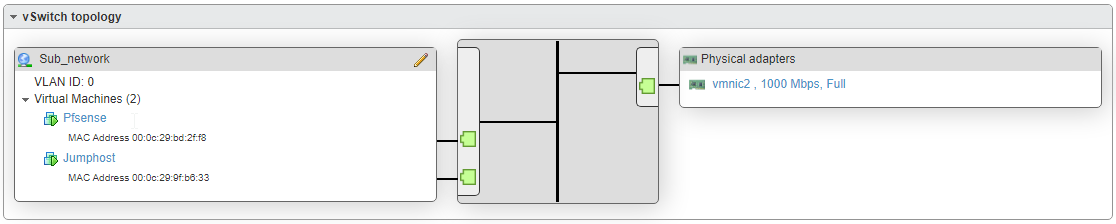
\includegraphics[width=0.9\textwidth]{Subswitch.png}
	\caption{Topologie van de 'Sub\textunderscore switch'}
	\label{fig:subswitch}
\end{figure}

\subsubitem{\bf Cisco\textunderscore switch}
\newline
Tot slot is er de 'Cisco\textunderscore switch' die gebruikt wordt om connectie te maken met alle apparaten, achterliggend de fysieke Cisco switch. Wanneer eindapparaten met de Cisco switch verbinden, zal de data passeren via de 'Cisco\textunderscore switch'. Op de figuur \ref{fig:Ciscoswitch} is ook te zien dat alle virtuele machines zich in deze omgeving bevinden. Dit zorgt ervoor dat de Cisco\textunderscore switch ingesteld is met vlan id 10, waarbij enkel data vanuit vlan 10 worden doorgestuurd naar de voorziene eindapparaten.

\begin{figure}[H]
	\centering
	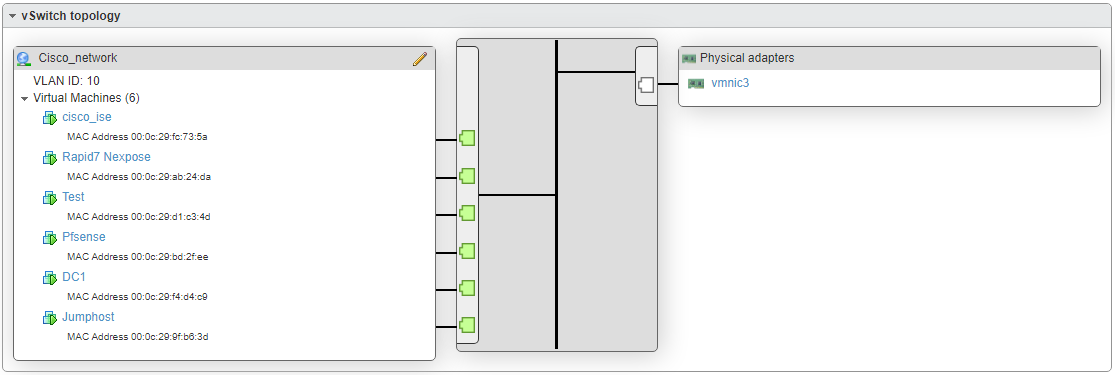
\includegraphics[width=0.9\textwidth]{CiscoSwitch_vmware.png}
	\caption{Topologie van de 'Cisco\textunderscore switch'}
	\label{fig:Ciscoswitch}
\end{figure}

\subsubsection{Server ESXi specificaties}
De VMware ESXi server is van het merk International Business Machines Corporation, gekend als IBM. Deze server werd oorsprongelijk gebruikt in de productieomgeving van Axians, maar wordt sinds kort als test server gebruikt. In figuur \ref{fig:VmwareSer} ziet men een afbeelding van de IBM ESXi server.
\newline
\newline
Het model van de VMware ESXi server is ‘System x3350 M3’ dat gekend staat binnen Axians als ‘de oude shr-esx-04 server’. De IBM ‘System x3350 M3’ bevat volgende specificaties:


\begin{itemize}
	\item Vormfactor: 1U Rack
	\item Processor:
	\begin{itemize}
		\item Proccessorsnelheid: 2.53GHz
		\item Processor: 6-core processor
	\end{itemize}
	\item Geheugen:
	\begin{itemize}
		\item Intern geheugen: 240 GB Random Access Memory
		\item Intern geheugentype: Double Data Rate 3 Synchronous Dynamic Random-Access Memory, gekend als DDR3 SDRAM
	\end{itemize}
	\item Opslag:
	\begin{itemize}
		\item Maximum aantal schrijven: 8 Slots
		\item Opslag: 4 Terabyte HHD 7500 RPM
	\end{itemize}
	\item Netwerk
	\begin{itemize}
		\item Ethernet interface type: Gigabit Ethernet
		\item Aantal Ethernet poorten: 4 
	\end{itemize}
\end{itemize}

\begin{figure}[H]
	\centering
	\includegraphics[width=0.7\textwidth]{serveresxi.png}
	\caption{Foto van de ESXi VMware server}
	\label{fig:VmwareSer}
\end{figure}
\newpage
\subsection{Cisco switch}
Naast de VMware ESXi server, bestaat de Cisco Identity Services Engine omgeving ook uit een Cisco switch. Op figuur \ref{fig:switch} ziet men een foto van de Cisco switch. Dankzij een aantal configuraties op de Cisco switch kan de Cisco Identity Services Engine virtuele machine communiceren met de fysieke switch. Deze noodzakelijke configuraties speelden een belangrijke rol in de configuratie van de Port-based network access control use case. 
\newline
\newline
Door een aantal basis configuraties op de switch uit te voeren, wordt communicatie tussen het afgezonderd netwerk en de eindapparaten die zich achter de Cisco switch bevinden ook mogelijk. Deze informatie is in sectie \ref{sec:config} terug te vinden.


\subsubsection{Configuratie}
\label{sec:config}
Vooreerst zijn een aantal commando's uitgevoerd die het netwerk apparaat beveiligen met een secret, line passwords en password encryption om inbreuk tegen te gaan. Vervolgens werd Gigabit Ethernet 0/1 geconfigureerd met de gepaste trunk instellingen om een gobale communicatie mogelijk te maken. Een trunk configuratie maakt data overdracht van de verschillende vlan's mogelijk. Volgende twee trunk commando's zijn hiervoor uitvoerd:  

\begin{itemize}
	\item switchport mode trunk
	\item switchport trunk allow vlan 10 
\end{itemize}

Gigabit Ethernet 0/1 werd rechtsverbonden met één van de interfaces op de VMware ESXi server, waarbij de virtuele switch ingesteld werd met vlan id 0 dat gelijk staan aan geen vlan identificatie. Vervolgens werd
op de Cisco switch vlan 10 gecreeërd met ip adres '192.168.17.5' en met subnet mask '255.255.255.0'. Vermits de interface Gigabit Ethernet 0/1 geconfigureerd is om verbinding te maken met de VMware ESXi server, zijn de overige interfaces bedoeld voor de communicatie met de eindapparaten. 
\newline
\newline
Om de Port-based network access control use case te implementeren, werd een nieuw AAA model ingesteld. Dit AAA model werd vervolgens geïnitialiseerd met een radius server die gelijk staat aan het Internet Protocol adres van Cisco Identity Services Engine. Ten slotte werd de dot1x aaa authentication methode met zijn standaard netwerk groep mee configureerd. 
\newline
\newline
Om de configuraties van de Cisco switch te beëindeigen, werd dot1x system-auth-control vastgelegd en werden alle interfaces voorzien van de nodige Port-based network access control configuraties. Figuur \ref{fig:RunningConfig} toont de running config van de Switch Cisco, daarnaast zijn alle nodige commando's in onderstaande lijst weergegeven.

\begin{itemize}
	\item \#enable
	\item \#config t
	\item (config)\#aaa new-model
	\item (config)\#aaa group server radius ISE
	\item (config-sg-radius)\#server-private 192.168.17.4 key Admin2020
	\item (config-sg-radius)\#exit
	\item (config)\#aaa authentication dot1x
	\item (config)\#aaa authorization network default group ISE
	\item (config)\#dot1x system-auth-control
	\item (config)\#interface range gig0/2-12
	\item (config-if-range)\#switchport mode access
	\item (config-if-range)\#switchmode access vlan 10
	\item (config-if-range)\#authentication host-mode multi-host
	\item (config-if-range)\#authentication port-control auto
	\item (config-if-range)\#dot1x pae auth
	\item (config-if-range)\#end
\end{itemize}

\begin{figure}[H]
	\centering
	\subfloat{{\includegraphics[width=4cm]{Switch_config1.png} }}%
	\qquad
	\subfloat{{\includegraphics[width=4cm]{Switch_config2.png} }}%
	\qquad
	\subfloat{{\includegraphics[width=4cm]{Switch_config3.png} }}%
	\caption{Running config van de Cisco switch}%
	\label{fig:RunningConfig}%
\end{figure}
Verder zijn 1G cat5e Ethernet kabels gebruikt om de hardware componenten met elkaar te laten communiceren. De Unshielded Twisted Pair Ethernet kabels halen snelheden tot 1000 Mbit/s met een doorvoersnelheid van 100mhz wat geschikt is voor dit afgezonderd netwerk.

\subsubsection{Cisco switch specificaties}
De Cisco switch behoord tot de ‘Catalyst 2960-CX’ series die nu gekend staat binnen Axians als de ‘Demo switch’. Hierbij vindt men in onderstaande lijst de specificaties van de Cisco Catalyst 2960-CX serie switch:

\begin{itemize}
	\item Power over Ethernet:
	\begin{itemize}
		\item Ondersteunend: Ja
		\item Standaard: 802.3at (PoE+)
	\end{itemize}
	\item Netwerk:
	\begin{itemize}
		\item 8 Gigabit Ethernet aansluitingen
		\item 2 Gigabit Ethernet Copper uplinks
		\item 2 Gigabit Ethernet Small form-factor pluggable uplinks, gekend als SFP
	\end{itemize}
	\item Besturingsysteem/software:
	\begin{itemize}
		\item OS: Cisco IOS
    \end{itemize}
\end{itemize}

\begin{figure}[H]
	\centering
	\includegraphics[width=0.7\textwidth]{ciscoswitch.png}
	\caption{Foto van de Cisco switch}
	\label{fig:switch}
\end{figure}
\newpage
\subsection{Virtuele machines}
\subsubsection{Rapid7 Nexpose}
De Rapid7 Nexpose is een Windows Server 2019 datacenter virtuele machine dat in het bachelorproef.com domein werd toegevoegd. Op deze virtuele machine draait de Rapid Nexpose software genaamd InsideVM. Rapid Nexpose is een oplossing voor het kwetsbaarheidsbeheer die risico's analyseert over kwetsbaarheden, configuraties en controles. Gebruikers kunnen op hun manier kwetsbaarheden in besturingssystemen, software van derden, webapplicaties, browsers en databases efficiënt beheren en problemen met verkeerde configuratie identificeren(\cite{Rapid7Li}). De Rapid7 Nexpose virtuele machine werd specifiek gebruikt in combinatie met de Cisco Identity Services Engine virtuele machine voor de Thread-Centric network access control use case. Op figuur \ref{fig:nexpose} is de home pagina van InsideVM weergegeven die u een visueel beeld geeft van de Rapid7 Nexpose software.
\newline\newline
Daarnaast werd de virtuele machine voorzien van de volgende specificaties: 
\begin{itemize}
	\item Geheugen: 48 GB Random Access Memory
	\item Opslag: 356 GB
	\item CPU: 24 cores
	\item Netwerk adapter: Cisco\textunderscore netwerk
\end{itemize}

Meer informatie over de installatie van Rapid7 Nexpose kan men op de website van Rapid7 terugvinden (\cite{rapid7}).

\begin{figure}[H]
	\centering
	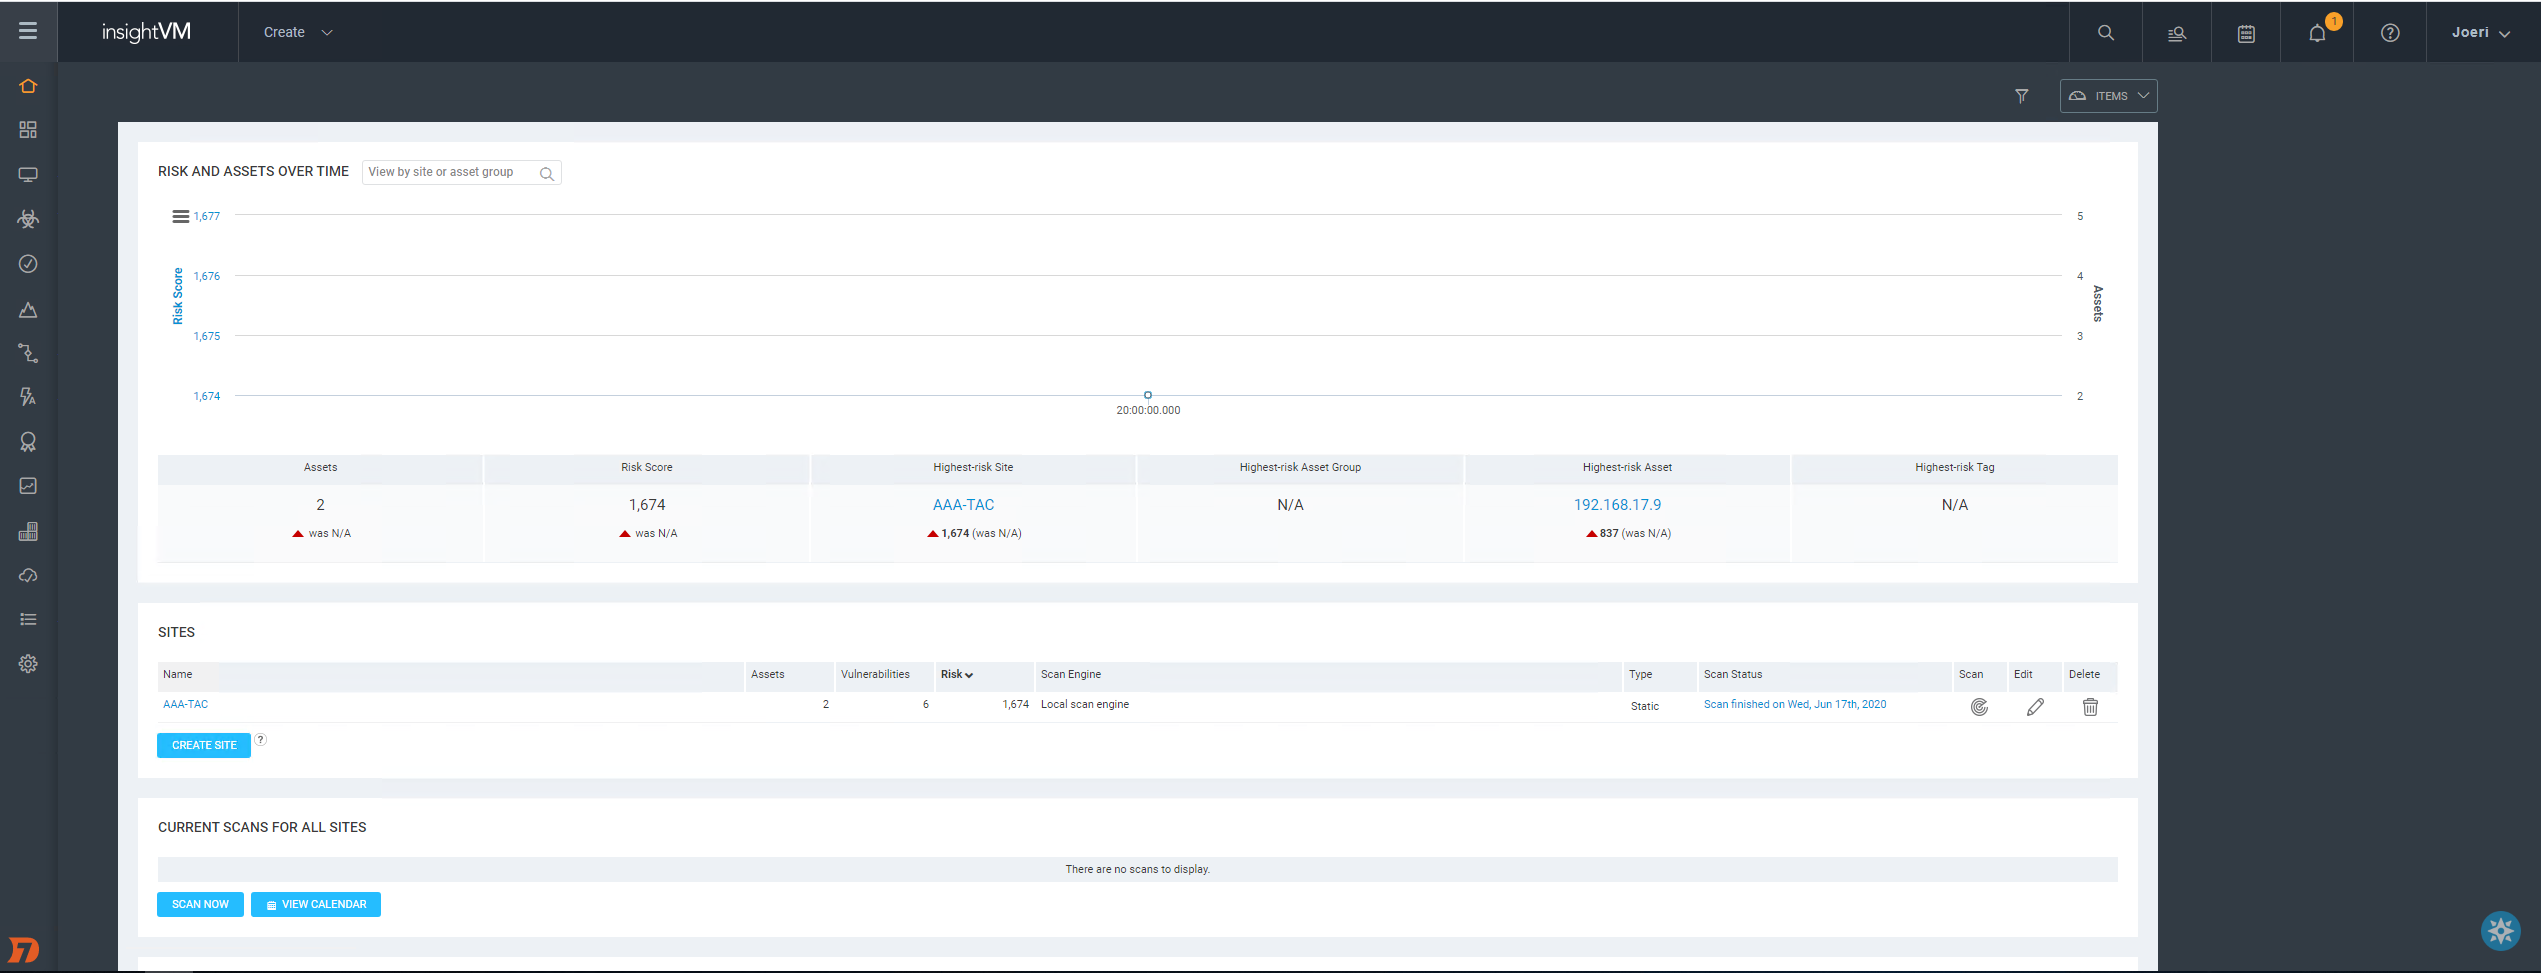
\includegraphics[width=1\textwidth]{nexpose.png}
	\caption{Home pagina van InsideVM}%
	\label{fig:nexpose}%
\end{figure}
\newpage
\subsubsection{Cisco Identity Services Engine}
De tweede virtuele machine waar dieper wordt op ingegaan, is Cisco Identity Services Engine. Deze virtuele machine zal zich verdiepen in de use cases: Port-based, Policy-based en Thread-centric network access control. Daarvoor zijn een aantal configuraties uitgevoerd op de virtuele machine van Cisco Identity Services Engine om een antwoord te geven op het onderzoek. Hieronder worden de configuraties opgesplitst per use case waarbij de use cases in de praktijk vaak worden gecombineerd. De resultaten van de Cisco Identity Services Engine configuraties vindt men terug in Hoofdstuk \ref{ch:Resultaten}.
\newline
\newline
Alvorens men dieper ingaat op de use cases werd Cisco Identity Services Engine toegevoegd aan het Active Directory Domain. Figuren \ref{fig:AD_Cisco1} en \ref{fig:AD_Cisco2} tonen aan dat de virtuele machine van Cisco Identity Services Engine probleemloos toegevoegd is aan het domein 'Bachelorproef.com'. Dit toont aan dat Cisco Identity Services Engine eenvoudig geïntegreerd kan worden met een domein waarbij extra policy rules in de toekomst kunnen worden ingevoerd. Dit onderzoek focust zich op de bescherming van de beschikbare interfaces op de Cisco switch, dit door een extra authenticatie methode te voorzien en dus niet door een integratie van Port-based network access control met het gebruik van Active Directory Domain users.

Verder werd systeem geïnstalleerd op een Red Hat Enterprise 7 distributie, waar volgende specificaties zijn voor vrijgemaakt: 

\begin{itemize}
	\item Geheugen: 128 GB Random Access Memory
	\item Opslag: 512 GB
	\item CPU: 24 cores
	\item Netwerk adapter: Cisco\textunderscore netwerk
\end{itemize}

De installatie van Cisco Identity Services Engine werd mogelijk door \cite{CiscoISE_InstallationGuide}.

\begin{figure}[H]
	\centering
	\includegraphics[width=1\textwidth]{AD_ise.png}
	\caption{Cisco ISE gelinkt met het AD domein}%
	\label{fig:AD_Cisco1}%
\end{figure}

\begin{figure}[H]
	\centering
	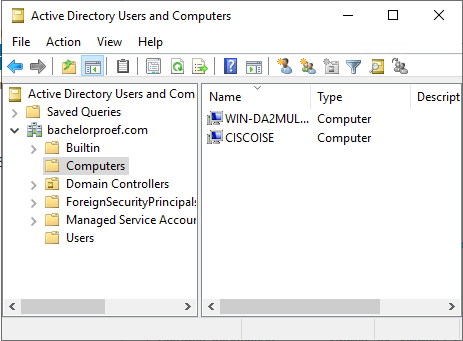
\includegraphics[width=0.8\textwidth]{ADComputers.png}
	\caption{Active Directory Users en Computers}
	\label{fig:AD_Cisco2}
\end{figure}

\fontsize{12}{20}\textbf{Port-based en Policy-based network access control }
 \newline
\newline
	Eerder werd vernoemd in sectie \ref{sec:config} dat implementatie van de Port-based network access control configuraties op de Cisco switch verplicht zijn. In dit onderdeel van de sectie ligt de focus op de configuratie van de Port-based network access control use case in de Cisco Identity Services Engine webbrowser. 
	\newline
	\newline
	De configuratie wordt gestart met de creatie van een aantal Cisco Identity Services Engine users in het 'Identity Management' tabblad. In figuur \ref{fig:users} ziet men twee aangemaakte users waarbij user 'TestV2' zich in de groep 'Employees' bevindt en user 'Test' niet. Dit zal zich uiten wanneer een gebruiker zich aanmeldt met de user 'Test'. Hierbij zal hij geen toegang krijgen tot het netwerk aan de hand van een beleidsregel.
 	\begin{figure}[H]
 		\centering
 		\includegraphics[width=1\textwidth]{Port_users.png}
 		\caption{Cisco Identity Services Engine users}%
 		\label{fig:users}%
 	\end{figure}
 Vervolgens werd in het tabblad 'Network Resources' de Cisco switch vastgelegd waardoor Cisco Identity Services Engine communicatie met het netwerk apparaat kan vaststellen. Figuur \ref{fig:ISESwitch} toont de configuratie voor deze communicatie. 
 	
 	 	\begin{figure}[H]
 		\centering
 		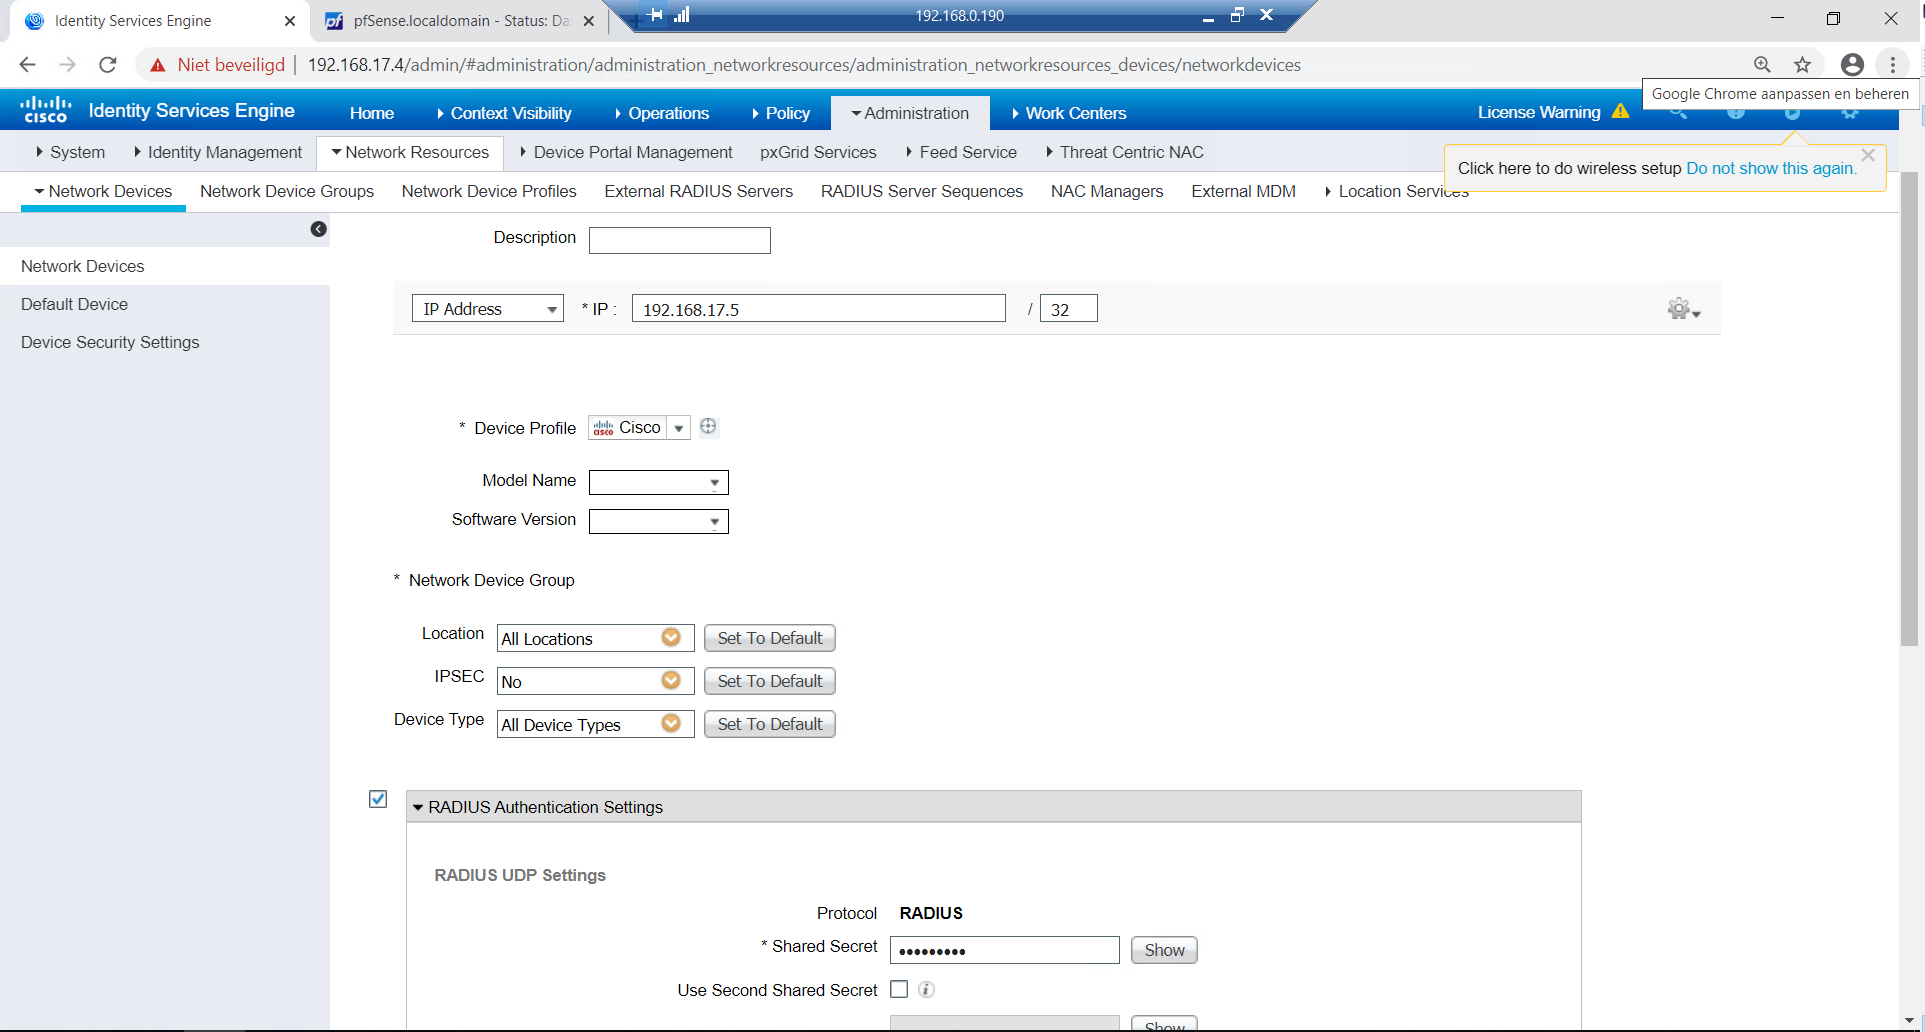
\includegraphics[width=0.9\textwidth]{ISESwitch.png}
 		\caption{Configuratie van de Cisco switch in ISE}%
 		\label{fig:ISESwitch}%
 		\end{figure}
 	
 	Daarbovenop is een beleidsregel ingesteld waarbij gecontroleerd wordt of de gegevens overeenkomen met de instellingen van de beleidsregel. In dit geval laat de beleidsregel netwerk verkeer toe als de gebruiker de juiste identificatie gegevens ingeeft, maar anderzijds moet de gebruiker ook tot de groep 'Employees' toegewezen zijn. Op figuur \ref{fig:ISESwitch} is de beleidsregel weergegeven.
 	
	 	 \begin{figure}[H]
		\centering
		\includegraphics[width=0.9\textwidth]{PolicySet_Port.png}
		\caption{Configuratie van de 802.1x policy rule in ISE}%
		\label{fig:ISESwitch}%
		\end{figure}
	\newpage
	Om de Port-based en Policy-based network access control use case uit te breiden werd een 'Authorization Policy - Global Exceptions' ingevoerd zodat toegang op het netwerk met een Ethernet kabel vanuit de Cisco switch enkel mogelijk is op bepaalde weekdagen. Zo kunnen bedrijven een beleidsregel implementeren die de toegang naar het netwerk op weekend dagen blokkeert. Op figuur \ref{fig:weekend} is de Global Exceptions beleidsregel terug te vinden waarbij men de beleidsregel test in Hoofdstuk \ref{ch:Resultaten}. 
	
	\begin{figure}[H]
		\centering
		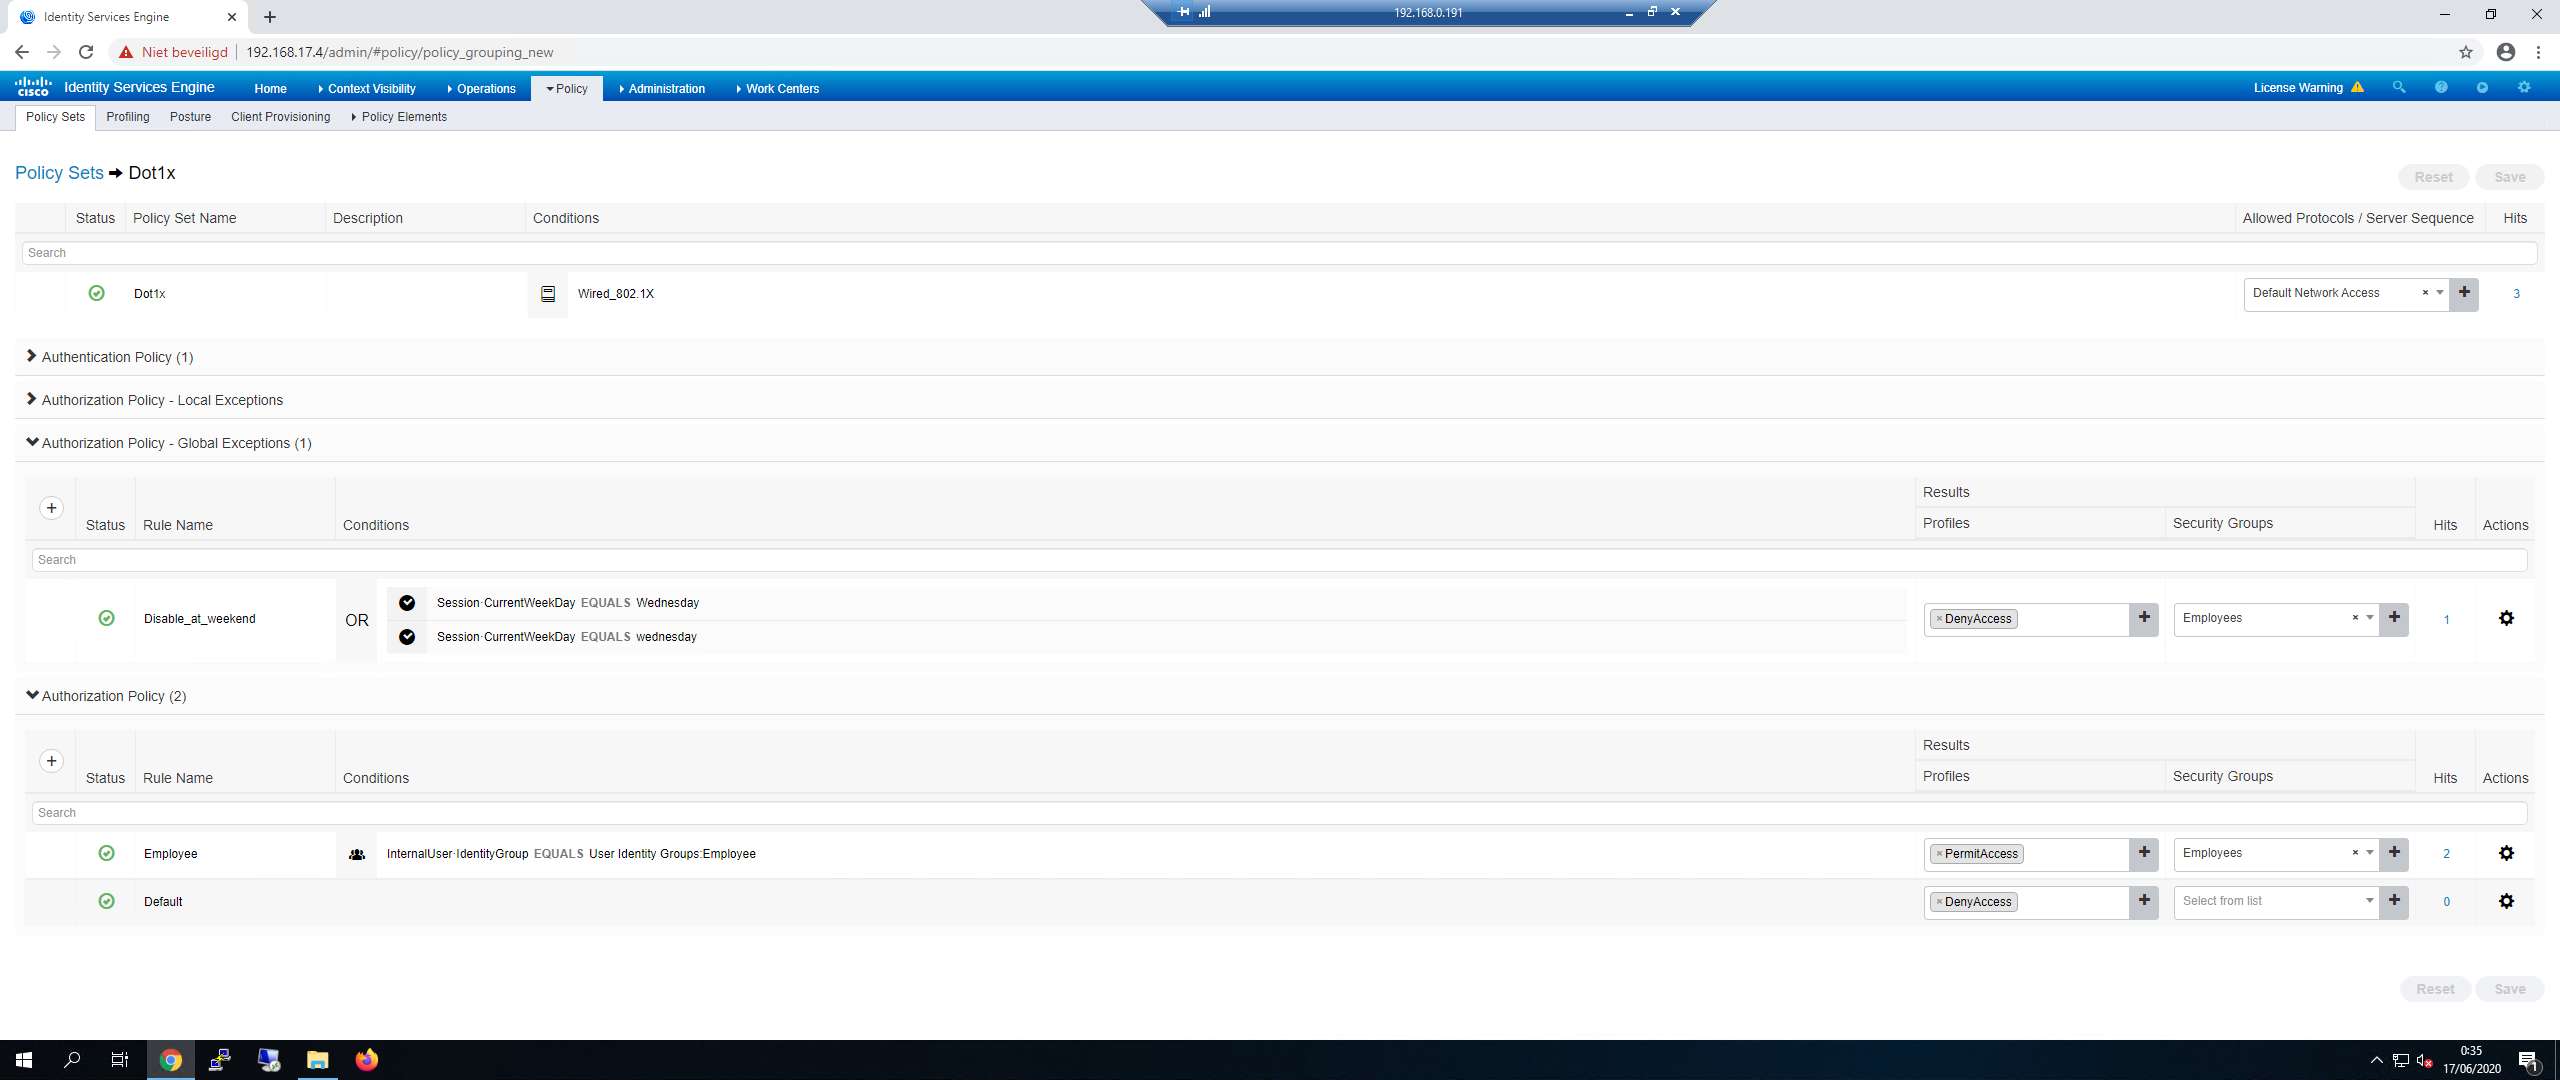
\includegraphics[width=1\textwidth]{Disable_At_Weekend_policy.png}
		\caption{Configuratie van de 802.1x weekend policy rule in ISE}%
		\label{fig:weekend}%
	\end{figure}
\fontsize{12}{20}\textbf{Thread-Centric en Policy-based network access control }
 \newline
 \newline
 In dit onderdeel van Cisco Identity Services Engine ligt de focus op de Thread-Centric en Policy-based network access control use case. Zoals voordien vermeld zijn de laatstgenoemde use cases gecombineerd omdat de Thread-Centric network access control use case gebruikmaakt van policy rules. Hiervoor werd Rapid7\textunderscore nexpose als Thrid Party Vendor gebruikt(\cite{rapid7}).
 \newline
 \newline
 Om de configuratie van Thread-Centric network access control te starten wordt de 'Thread-Centric NAC service' ingeschakeld. Op figuur \ref{fig:serviceThread} is te zien dat de service in \textbf{Administration > System > Deployment} werd ingeschakeld.
 
\begin{figure}[H]
		 	\centering
		 	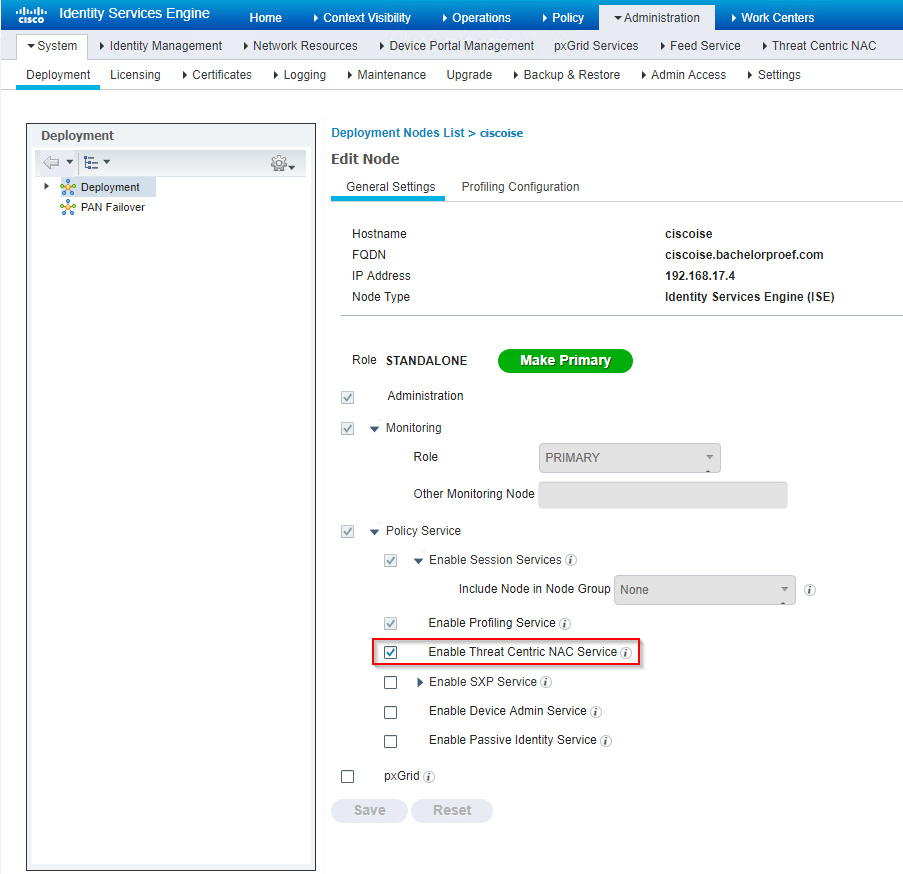
\includegraphics[width=0.9\textwidth]{threadcentricService.png}
		 	\caption{Thread-centric NAC service in ISE}%
		 	\label{fig:serviceThread}%
\end{figure}

 Vervolgens werden de certificaten tussen Cisco Identity Services Engine, Windows Active Directory en Rapid7 Nexpose geconfigureerd. Indien men meer informatie wenst over de configuratie van deze certificaten kan men \cite{thread_yt} bekijken.
 \newline
 \newline
 Als volgt zijn er een aantal instellingen uitgevoerd op de Rapid7 Nexpose applicatie zoals de creatie van een site die de assets bevat. In dit geval werd een laptop die reeds verbonden was met het afgezonderd netwerk gebruikt als asset. Op het eind van de configuratie zal Cisco Identity Service Engine een automatische scan uitvoeren wanneer de laptop zich aansluit op het netwerk. 
 \newline
 \newline
 Communicatie tussen Cisco Identity Services Engine en Rapid7 Nexpose werd mogelijk door een 'Vendor Instance' aan te maken. Op figuur \ref{fig:vendor} is de configuraties van de 'Vendor Instance' weergegeven.
	 \begin{figure}[H]
		 	\centering
		 	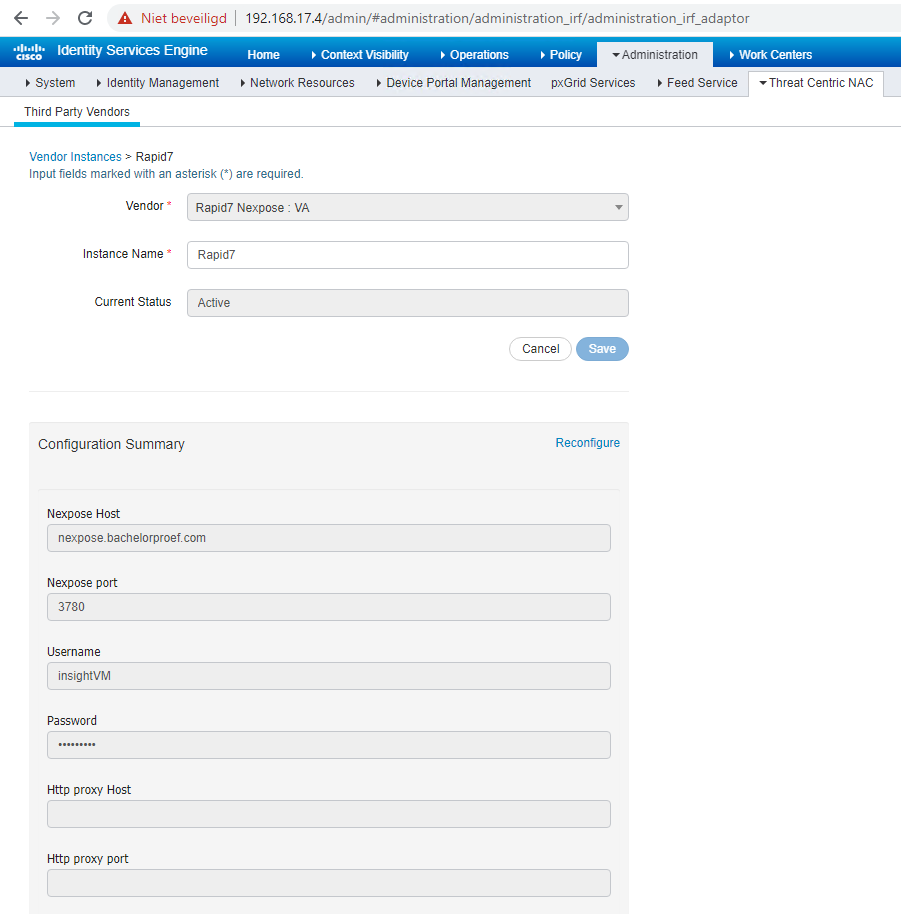
\includegraphics[width=0.9\textwidth]{VendorRapid7.png}
		 	\caption{Rapid7 Vendor Instance in ISE}%
		 	\label{fig:vendor}%
	 \end{figure}
Nadien werden er Authorization Profiles aangemaakt die een Rapid7 Nexpose scan triggeren. Dit werd mogelijk door te navigeren naar \textbf{ Policy > Policy Elements > Results > Authorization > Authorization Profiles}. Er werden twee Authorization Profiles aangemaakt namelijk: 'WIRED\textunderscore VA\textunderscore USER' en 'WIRED\textunderscore VA\textunderscore QUARANTINE'. 
 \newline
\newline
Wanneer een eindapparaat verbinding maakt met het netwerk langs de Cisco switch dan wordt het eindapparaat via 'WIRED\textunderscore VA\textunderscore USER' toegewezen. Vervolgens wordt een automatische scan gestart in Rapid7 Nexpose die getriggerd wordt door Cisco Identity Services Engine. 
 \newline
\newline
Indien het eindapparaat een bepaalde 'Nexpose-CVSS\textunderscore Base\textunderscore Score' heeft, zal afhankelijk van de score het eindapparaat het 'WIRED\textunderscore VA\textunderscore QUARANTINE' Authorization Profile toegewezen krijgen. Dit resulteert in een eindapparaat dat geen toegang meer heeft tot het netwerk. Figuur \ref{fig:WIRED} toont één configuratie van de Authorization Profiles namelijk de WIRED\textunderscore VA\textunderscore USER. 
\newline
\newline
Belangijk om te weten is dat de 'WIRED\textunderscore VA\textunderscore USER' Authorization Profile de volgende 'Attributes Details' kent: 
	\begin{itemize}
	\item Access Type = ACCESS\textunderscore ACCEPT
	\item on-demand-scan-interval = 48
	\item periodic-scan-enabled = 24	
	\item va-adapter-instance = (Instance-id van de 'Adapter Instance')
\end{itemize}

 \begin{figure}[H]
	 	\centering
	 	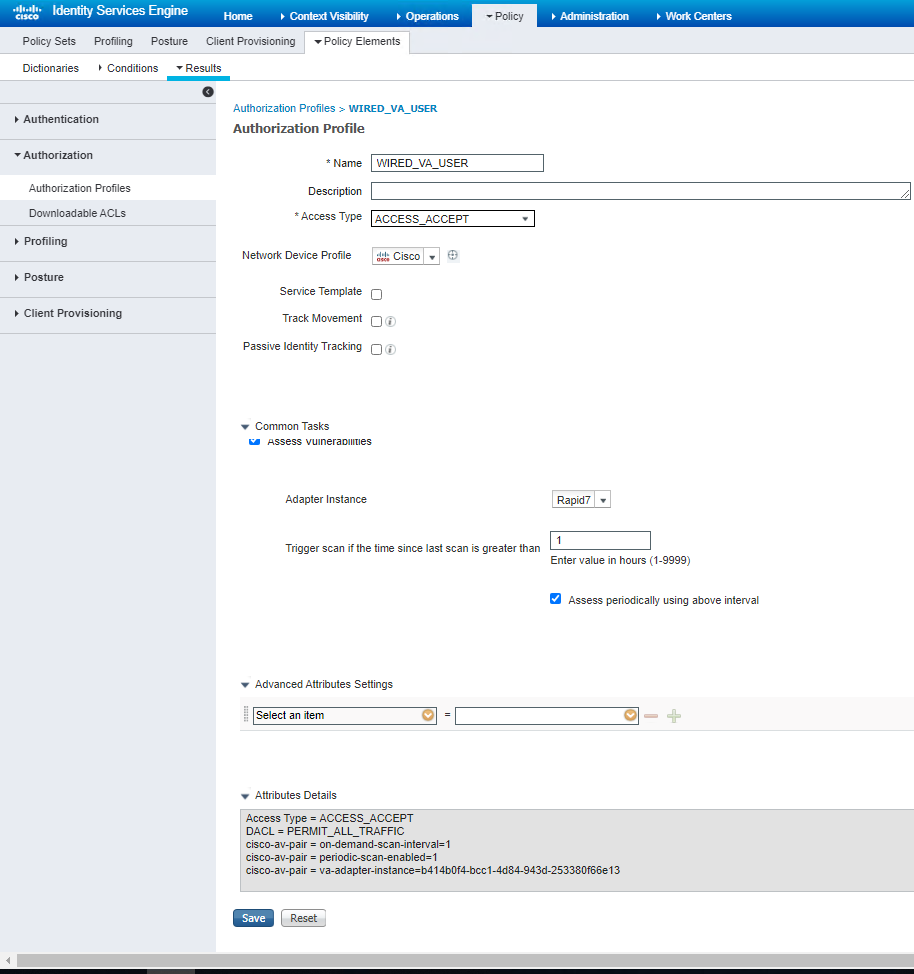
\includegraphics[width=0.9\textwidth]{WIRED7.png}
	 	\caption{Authorization Profile WIRED\textunderscore VA\textunderscore USER}%
	 	\label{fig:WIRED}%
 \end{figure}

Tot slot zijn er nog de policy rules die eindapparaten toelaten of in
quarantaine plaatsen. Op figuur \ref{fig:quarin} ziet men de policy rules die geïmplementeerd zijn voor het Thread-Centric network access control use case. Hierbij werd de Dot1x beleidsregel aangepast zodanig dat de Profile Results gebruikmaakt van 'WIRED\textunderscore VA\textunderscore USER'. Daarnaast werd er een 'Authorization Policy - Global Exceptions' ingevoerd die eindapparaten in quarantaine plaatsen indien het rapport van Rapid7 Nexpose uitwijst dat het eindapparaat een Nexpose-CVSS\textunderscore Base\textunderscore Score heeft groter dan 4. 

  \begin{figure}[H]
 	\centering
 	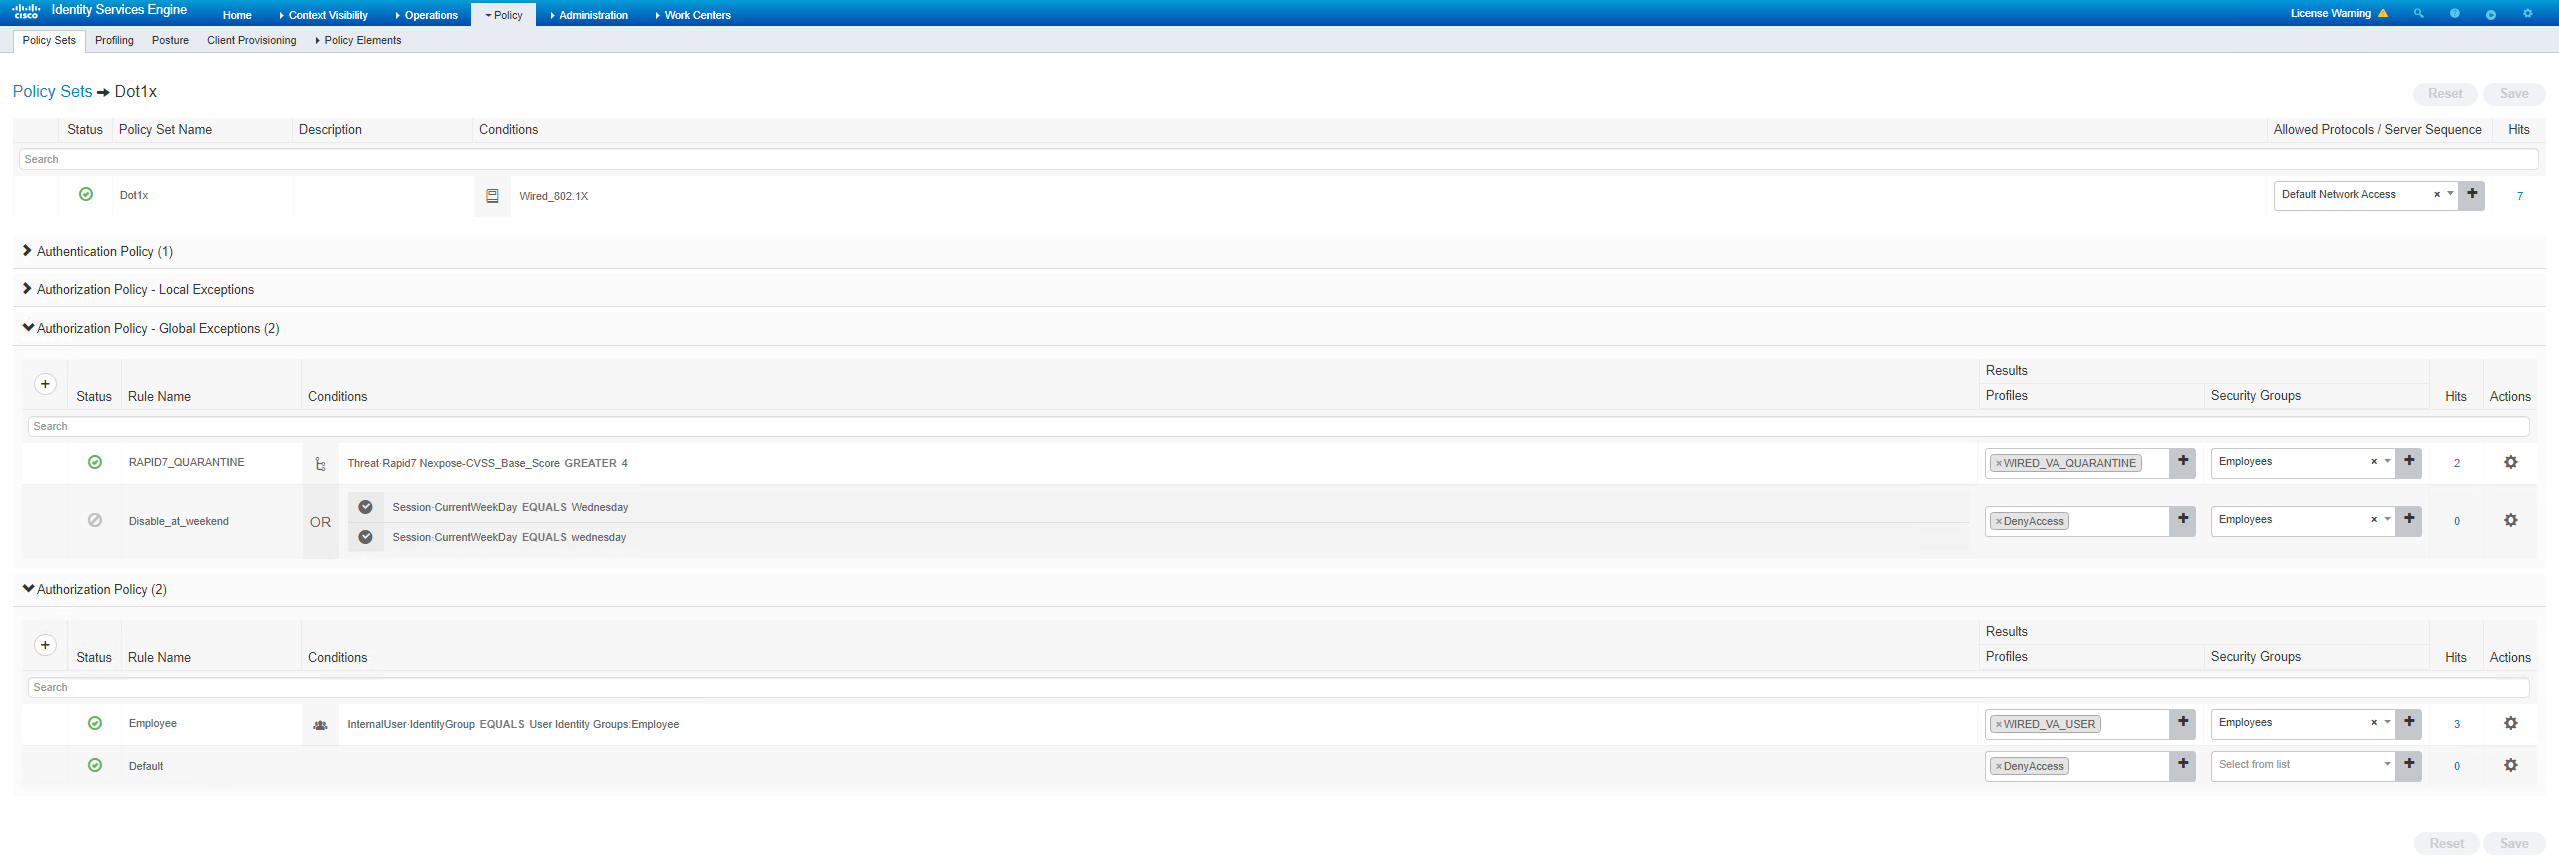
\includegraphics[width=1\textwidth]{PolicyRuleThreadCentric.png}
 	\caption{Policy rules Thread-Centric NAC in ISE}%
 	\label{fig:quarin}%
 \end{figure}
 
 De installatie van Thread-Centric network access control in combinatie met Rapid7 Nexpose werd mogelijk door \cite{thread_yt}.

 
\subsubsection{Windows server 2019 datacenter domeincontroller}
Het gebruik van een Windows Server 2019 maakt de creatie van een Active Directory domein mogelijk. Een nieuwe forest werd hiervoor aangemaakt en de Windows Server 2019 werd meteen ook gepromoveerd naar de domeincontroller binnen het 'bachelorproef.com' domein.
\newline
\newline
Via Cisco Identity Service Engine kan men subset van domeinen selecteren vanuit de vertrouwde domeinen voor authenticatie en autorisatie. Deze subset van domeinen worden authenticatiedomeinen genoemd. Het definiëren van deze authenticatiedomeinen verbetert de beveiliging voor bepaalde domeinen, waardoor de authenticatie van de gebruikers op deze domeinen wordt beperkt(\cite{winISE}).
\newline
\newline
Zoals voorheen vermeld, is integratie met Windows Server Active Directory en Cisco Identity Services Engine reeds mogelijk. Hierdoor kunnen bedrijven met Cisco Identity Services opteren om werknemers te laten inloggen op het netwerk met de 'Domain Users’. Vaak wordt deze methode geïntegreerd met het 802.1x wireless Port-based network access control use case om zich aan te melden op het netwerk met gebruik met de Active Directory Domain gegevens. Helaas beschikte dit afgezonderde netwerk niet over een wireless controller die dit mogelijk maakt. Cisco Identity Services voorziet hiervoor vooraf gedefinieerde regels.

Verder wordt het ‘Remote Desktop Protocol (RDP)’ in combinatie met het Internet Protocol (IP) adres gebruikt om de Windows machines te bereiken.
\newline
\newline
Om de Windows server 2019 datacenter te gebruiken werden volgende specificaties vrijgemaakt:

\begin{itemize}
	\item Geheugen: 16 GB Random Access Memory
	\item Opslag: 126 GB
	\item CPU: 20 cores
	\item Netwerk adapter: Cisco\textunderscore netwerk
\end{itemize}

Als laatsts werd de installatie van Windows Server 2019 datacenter mogelijk door \cite{Win19_InstallationGuide}. 

\subsubsection{Pfsense}
De Pfsense virtuele machine verwijst naar de virtuele router waarbij één interface van de Pfsense gebruikt wordt als gateway voor alle vlan’s en van alle componenten die zich achter de Cisco switch bevinden. Vervolgens wordt de WAN interface van de Pfsense gebruikt om de data van en naar de Local Area Network interface te sturen. Hierdoor is er communicatie vanuit het thuisnetwerk met het afgezonderd netwerk mogelijk.
\newline
\newline
De pfsense is enkel te contacteren binnen het afgezonderd netwerk door ‘Hypertext Transfer Protocol (HTTP)’ te gebruiken. Met andere woorden kunnen enkel machines in het netwerk '192.168.17.0/24' de Pfsense interface bereiken door te surfen naar het ip-adres: '192.168.17.1'. Op figuur \ref{fig:Pfsense} is te zien dat de home interface van de Pfsense te bereiken is via 'http://192.168.17.1/'.
\newline
\newline
Ten slotte werd dit systeem geïnstalleerd op een Free Berkeley Software Distribution, waarvoor volgende specificaties zijn voor vrijgemaakt:  

\begin{itemize}
	\item Geheugen: 4 GB Random Access Memory
	\item Opslag: 25 GB
	\item CPU: 4 cores
	\item Netwerk adapter: Cisco\textunderscore netwerk
\end{itemize}
De installatie van Pfsense werd door \cite{Pfsense_InstallationGuide} mogelijk gemaakt.

\begin{figure}[H]
	\centering
	\includegraphics[width=0.9\textwidth]{PfsenseHome.png}
	\caption{Home webinterface van Pfsense}
	\label{fig:Pfsense}
\end{figure}

\subsubsection{Jumphost}
Een jumphost is een tussenliggende host machine waarbij connectie naar een extern netwerk mogelijk is. Vervolgens kan een verbinding worden gemaakt met een andere host in het extern netwerk. Met andere woorden 'jumpt' men dus van het ene apparaat naar het andere om een extern netwerk te bereiken. 
\newline
\newline
Dit werd in de Cisco Identity Services Engine omgeving ook gebruikt waarbij een eindapparaat in het thuisnetwerk verbinding maakt met de Jumphost via Remote Desktop Protocol om zo eindapparaten in het afgezonderd netwerk te contacteren. Hierbij zijn volgende instellingen gebruikt:  
 
 
\begin{itemize}
	\item Geheugen: 16 GB Random Access Memory
	\item Opslag: 126 GB
	\item CPU: 20 cores
	\item Netwerk adapter 1: Cisco\textunderscore netwerk
	\item Netwerk adapter 2: Sub\textunderscore netwerk
\end{itemize}

De installatie van de Jumphost werd door \cite{Win19_InstallationGuide} mogelijk. 

\section{Cisco Identity Services Engine enquête}
\label{sec:enquête}
Om een link te leggen met de resultaten van de uitgevoerde proeven, werd een enquête opsteld. Deze enquête wordt als onderliggende basis gebruikt bij de analyse van de resultaten die verkregen werden door de fysieke proeven. Zoals in vorige hoofdstukken vermeld, is deze enquête een opiniepeiling waarbij een aantal vragen gesteld zijn aan personen die reeds bekend zijn met Cisco Identity Services Engine. Hierdoor is de doelgroep van deze enquête beperkt tot de Cisco Identity Services Engine specialisten.
\newline
\newline
De enquête is publiekelijk gemaakt via LinkedIn en via E-mail. Linkedin is een online sociaal netwerk dat is opgericht voor vakmensen, die ongeveer 610 miljoen geregistreerden telt(\cite{LinkedTIN}). Omdat deze enquête publiekelijk werd gemaakt op \cite{LinkedIn}, bevat dit formulier een aantal ‘failsave’ vragen. Deze ‘failsave’ vragen zijn bedoeldt wanneer niet Cisco Identity Services Engine specialisten de enquête proberen in te vullen. Met als gevolg dat de kans op onjuiste ingevulde antwoorden verkleind werd.
\newline
\newline
Dit formulier werd mogelijk gemaakt door Microsoft en Hogeschool Gent. Elke student heeft recht op een gelicentieerd Office 365 pakket gedurende zijn opleidingstraject. Het programma in kwestie noemt men \cite{MicrosoftForms} dat standaard inbegrepen is in het Microsoft Office 365 pakket.
\newline
\newline
Een overzicht van de vragen die gesteld werden tijdens de enquête is terug te vinden in bijlage \ref{ch:Resultaten_enquête}.


